\section{Overview}
\label{sec:overview}
%In this section, we provide our assumptions, a description of the design, a simple example to explain how our solution works, and enumerate the advantages of the system.
This section presents the motivation, design and advantages of a location disclosure system based on keywords. 

\subsection{A keyword-based solution}
\label{subsec:key}

% Location information\footnote{we focus on location information that can be collected via mobile devices} 
% has the following properties: 
% (i) it is considered more sensitive than other types of personal information and more valuable, 
% (ii) its utility is transient in many cases;
% for targeting reasons knowing real-time location is often more useful than knowing location later, 
% (iii) it is predictable; mobility patterns have been shown to be periodic~\cite{salva}.  

Our requirements calls for a solution to share information about location monetized by ad-networks and 3rd party aggregators through \emph{selective disclosure}. For the user to retain control, our privacy solution should address \emph{how} the information is released, under \emph{which conditions} the information is released and to \emph{whom}, as seen in previous ones, e.g.~Koi~\cite{guha:koi}, 

% To meet our requirements, we create a solution based around \emph{selective disclosure}; users disclose location information that they are willing 
% to release.
% This information is monetized by ad-networks and third party aggregators by way of online ads. 
% The control remains with the user. 
% Any privacy solution based around selective disclosure 
% needs to
% address 
% \emph{how} the information is released, under \emph{which conditions} the information is released and to \emph{whom}.

To specify \emph{how} and \emph{under which conditions} location information is released, we choose to use keywords. 
While the information that is released is a latitude longitude pair (lat-long), the decision to disclose is based on associated keywords. 
Users who are comfortable disclosing location under certain circumstances~\cite{Kelley:2011} opt-in to reveal lat-long associated with keywords of their choices.
%
% In order to answer \emph{how} we release location information, we design our solution around keywords
% associated with locations; the decision to release is based on keywords associated with locations, and
% the information that is actually released is the location. %% IS IT THE LOCATION, OR THE KEYWORD?
An example would be a street that has many restaurants serving different cuisines, it would have keywords like ``restaurant, Thai, French, Indian'' associated each with the lat-long of each particular venue. 
The use of keywords brings important advantages: 
(i) Keywords let us deal with the problem of location privacy at a higher abstraction than coordinates or even location descriptors as in Koi~\cite{guha:koi}. 
(ii) Keywords are user friendly: instead of having to decide the sensitivity of every location, users decide on a much smaller set of keywords that they are comfortable releasing or not.
(iii) Today's ad-networks function primarily around keywords, thereby a solution around keywords can make it easier for ad-networks to adopt and use.
(iv) As there can be a finite set of keywords associated with any location, and the association of a keyword with a location typically remains for long periods of times, modifying keywords associated with a location is easy, making the solution scalable. 

Our solution compensates users \emph{economically} for information they release to aggregators and ad-networks. Economic incentives can nudge more users towards adoption, as concerns about privacy alone are rarely sufficient. Concrete incentives also sometimes reduce users' cognitive biases when it comes to perceiving their privacy~\cite{loewenstein2010misplaced}. Specifying to \emph{whom} the information is released is implicitly done by a market. 
%They also addresses the issue of to \emph{whom} the information will be released to -- parties that can pay. 
In principle, any parties that can pay for it is legitimate. In practice, this agreement should be facilitated by a trusted third party who vet the parties and send information about the user \emph{only} for locations she agreed on, upon payment. 

%At a high-level the core of our solution is based on involving the user in the economic value-chain
%that exists today around location information. The players that constitute this ecosystem include
%web content providers and application developers on one side whose respective offerings are often `free'. 
%On the other side are users who come attracted to the free offerings. 
%In addition, data aggregators
%and ad-networks who work with content providers and developers. 
%They collect information (including location) about users of applications and 
%monetize information by way of online ads. These ad-networks are in turn paid by advertisers. 
%A fraction of the revenue generated is passed on to
%application developers and content providers. 



% \textbf{Assumptions}
% As our solution is centered around economic transactions around location information, our architecture is designed for an honest-but-curious adversary. 
The design we next describe is meant to operate under the following set of \textbf{assumptions}. 
Given the amount of press on privacy related issues, we believe that the PR backlash in the case of a serious privacy violation will make such violations undesirable. As a consequence, we provision against an \emph{honest-but-curious} advertiser. It means the adversary complies with the system but it can exploit the information that is gathered for its own interest. We provide safeguards against inference and linkage attacks. We also assume that the mobile OS used complies with user's privacy, hence not sharing location information with any application once the user stated that request. 
Note that the architecture presented next is oblivious to a background service model (passive, potentially continuous tracking) or a check-in model. 

% Before describing the design, we first describe our \textbf{assumptions}.
% We consider our adversary to be an honest-but-curious advertiser. 
% This means our adversary participates in the system honestly but may try to exploit the information that is gathered.
% Hence our adversary is \emph{not} malicious. Applications leaking information to aggregators as well as aggregators involved
% in resale of data\footnote{like BlueKai~\url{http://www.bluekai.com/}} are not necessarily malicious, but honest but curious and economically motivated. 
% With this in mind, we provide safeguards against inference and linkage attacks.

% We provide safeguards against inference and linkage attacks. We do ensure that even if a link is established between a specific user and 
% a set of locations, no entity can gain economically with this information.

% We assume that once an entity enters into an agreement with the user, it is generally compliant. 
% We assume that location information can be tracked and gathered continuously, as this is the worst case. 
% In general this is not feasible as energy concerns around GPS usage will forbid this~\cite{energy:loc}. 


\subsection{Design and Example}
\label{subsec:design}

\begin{figure}[t]
	\begin{center}
		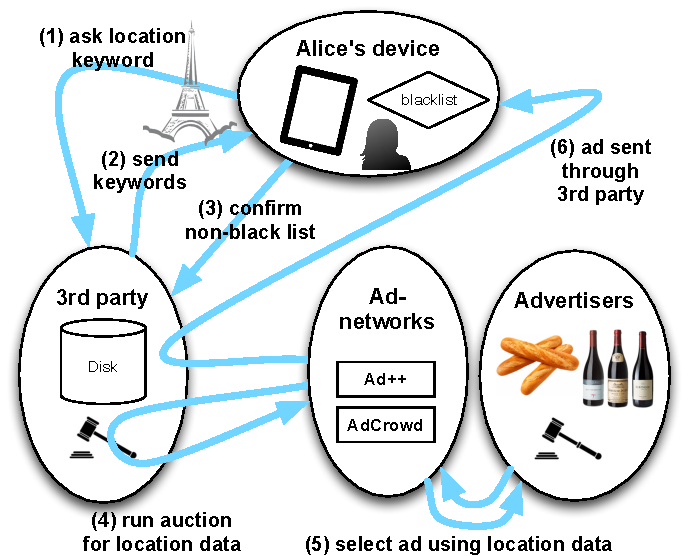
\includegraphics[width=0.9\linewidth]{fig/keyword/TLPOverview.pdf}
	\end{center}
	\caption{Solution overview}
	\label{fig:overview}
\end{figure}
The architecture consists of the following components: 
(i) a keyword server which maps physical locations to keywords
(ii) a location blacklist module which contains a list of sensitive keywords, 
communicates with the keyword server, and reveals non-sensitive locations
(iii) a blocking module in the network that blocks access to various parties, 
% (ii) a blacklist module that contains a list of sensitive keywords and maps these
% keywords to physical locations -- these are locations that will not be revealed, 
(iv) a market that puts up for sale information about locations visited by the user that are not in the blacklist, 
and (v) a module that grants \emph{access}
to the user for parties that pay, after purchasing access on the market.
With the exception of (ii), which can be a simple smartphone app, all modules are stored in the network; \emph{no} changes are required on the device.

A high-level diagram is shown in Fig.~\ref{fig:overview}. 
We describe the process with a simple example. 
Alice is willing to share certain locations and would like to hide her presence at other locations, a typical occurrence~\cite{Kelley:2011}. 
Alice wants to buy bread, shop for wine, and go to the Libertarian party headquarters. 
She would like to conceal her political leanings.
Alice would therefore put `Libertarian, Politics' as keywords in her \emph{blacklist module}. 
We describe in Sec.~\ref{subsec:implementation} how the blacklist formation can be simplified through nested menus and re-ordering. 
% This blacklist will be stored on a server at a third party location. 
We assume the third party is trusted and leave lowering this requirement to future work.

As Alice arrives at the bakery, her network activity goes through the \emph{blocking module} that runs a mix-network to conceal her real network address, and provides privacy protection like dropping cookies to third parties, overwriting \texttt{referer} headers etc.~\cite{Krishnamurthy:2007io} (see Sec.~\ref{subsec:implementation} for more on implementation).
At every location, Alice's device contacts the \emph{keyword server} which translates locations to keywords.
A check is then made against the blacklist to verify if Alice is comfortable releasing this information. 
If a location has multiple keywords and \emph{any} of them are on the blacklist, it is considered private.
% In order to perform this check, Alice's pwe need to translate the keywords to locations, described in Sec.~\ref{subsec:keywordmap}. 
Once a location passes the check, it is put on the \emph{market} for sale with a unique user-id and the keywords. 
This user-id is generated independently and can be periodically changed. 
The information then is ($UID_{Alice}$, (lat$_1$, long$_1$), Bakery). 
As she arrives at the wine shop, the information on the market will be ($UID_{Alice}$, (lat$_2$, long$_2$), Wine Shop), as the wine shop also passes the blacklist test. 
Ad-networks can pay to \emph{access} Alice based on these two locations released. 
The payment will be credited to Alice, with a small fraction taken by the third party. 
The third party then fixes a network address to reach Alice at the wine shop and conveys it to the ad-networks. 
Alice can receive a targeted ad (via an app or via SMS) for a particular wine.

As soon as Alice moves out of the wine shop, her network address changes and her location again is not known
to anyone but the trusted third party. 
When she is close to the Libertarian party headquarters, the check against the blacklist
returns a positive result, and this location is not revealed to anyone. 

% \subsection{Mapping Locations to Keywords}
% \label{subsec:keywordmap}
% Using a mapping of locations to keywords has a variety of challenges and advantages, which we now discuss.
% Locations may be defined in two ways which are both compatible with our system. It may denote a point of interest where users ``check in" (as in services like Foursquare) or alternatively it may represent a certain geographical area (defined using lat-longs or the coverage of a given cell tower).

% Creating a mapping of locations to keywords is not necessarily easy \emph{per se}, but one can reuse online services already providing such a mapping, such as Yelp, Google Places, and Foursquare.
% % This mapping can be obtained by gathering information from existing sites like Yelp, Google Places, or Foursquare.
% A ``folksonomy" approach could also be used where users augment the map over time, and even receive incentive. In this case, to encourage tagging of privacy-sensitive locations, the system can allow anonymous tagging. 
% Usability is also a challenge, and care must be taken to keep the number of keywords manageable and design the blacklist's user interface to be easy to use (see our UI in Sec.~\ref{subsec:implementation}).
% The keywords in the mapping will eventually be used by the user to specify a blacklist.
% Thus, 
% Yelp's hierarchical list of categories contains 885 entries, a reasonable number if handled properly in the UI.
% To specify a blacklist, a user need not look through every potential keyword. 
% Some ideas for the blacklist UI would be to group keywords into categories, where users can quickly decide if whole categories are sensitive or not, or can find specific words within a category that they think may be sensitive.
% % Rather, keywords can be grouped into categories, where users can quickly decide if whole categories are sensitive or not, or can find specific words within a category that they think may be sensitive.
% Additionally, categories that are more likely to be sensitive can be made more prominent in any blacklist creation software, by placing it at the beginning of a list, highlighting, etc. 


% \subsection{Design Specifics}
% \subsubsection{Blocking module}
% \label{sec:blocking}
% The purpose of this module is to block connections to prevent information leakage.
% Many mobile applications as well as web services rely on cookies to track the user,
% as well as send information to ad-networks and aggregators. 
% The connections to ad-networks and aggregators (AdMob, Flurry Analytics etc.) can be blocked by a proxy in the middle and by spoofing the MAC address. 
% All necessary proxies already exist: Privoxy comes with advanced filtering capabilities and handles rewrites of the HTTP headers like the `referrer' header to prevent leakages of any form, and mitmproxy can handle SSL\footnote{\url{www.privoxy.org}, \url{www.mitmproxy.org}}. 
% In addition, as the system works with opt-in users, we can have the users upload their SSH certificates to enable the module in the middle to masquerade as the user. 
% From an application's perspective, no logic is broken. 
% Even for location based services like Foursquare or maps, an unintentional checkin or a search at a private location can be prevented by checking against the blacklist -- an added benefit.  

% The proxy is part of a network of proxies that act as a mix network -- the real network address of the
%  mobile device will never be revealed to anyone. 

 %It is possible for manufacturers of mobile devices themselves
%to get information directly from the mobile device -- indeed Android seems to use SUPL to 

% \subsubsection{Blacklist module}
% \label{sec:blacklist}
% The objective of this module is to obtain the keywords for a user's current location, check the keywords against a blacklist, and then release the location if no keywords are blacklisted.
% The first step requires a mapping of locations to keywords.
% This mapping can be obtained by gathering information from Yelp, Google Places, or Foursquare.
% Additionally, a ``folksonomy" approach could be taken where users tag locations, building up a map over time.
% % Mention concern from paper: in folksonomy, sensitive places never covered?
% % In this case, users could again receive some incentive from 
% For simplicity and efficiency, the mapping of locations to keywords is on a central server.
% A user's blacklist is stored on her device, keeping this sensitive information away from a central point of attack.
% Encrypted queries from the device to the server in the form of lat-long coordinates will return keywords for that location.
% If no keywords exist for that location, a non-location-specific ad should be shown.
% The user's device can do a simple set intersection between the blacklist and the current location keywords and contact the ad-server accordingly.
% An open question is if zero-knowledge proofs can be used to notify a user of a location's keywords without the central server learning the user's location, thereby reducing the trust needed in the third party.

% A point of concern here is usability. 
% The number of possible keywords is probably on the order of 1000.
% To specify a blacklist, a user need not look through every potential keyword. 
% Rather, keywords can be grouped into categories, where users can quickly decide if whole categories are sensitive or not, or can find specific words within a category that they think may be sensitive.
% Additionally, categories that are more likely to be sensitive can be made more prominent in any blacklist creation software, by placing it at the beginning of a list, highlighting, etc.


\subsection{Summary of Advantages}
Now that we've described the system, we discuss the benefits of the system for various parties.
% There are benefits in the system for various parties.

\textbf{Users} obtain monetary payment for their data and privacy through choice.
The architecture operates in the network and hence, users do not need to make changes to their devices.
If information is leaked or shared between colluding ad-networks, these parties would have to gain access to the user to monetize this information -- and unless these parties have paid, they are prevented from gaining access to the user.
Hence, we protect against adversaries aiming to extract economic gain. 
We deal with adversaries who try to infer the identity of users or blacklisted keywords in Sec.~\ref{sec:security}.

The keyword system also benefits the user.
If a user is visiting a place they are unfamiliar with, they may not be accustomed to what areas are privacy sensitive.
Because keyword mappings work in any location, a user's privacy is protected even in unfamiliar areas.
Additionally, a user may simply not realize the privacy sensitive nature of a location they are in.
Because all traffic is directed through our system, if a user starts using a location-based service at a location they don't realize is privacy sensitive, our system can catch it and warn the user before they complete the action.

\textbf{Ad-networks and aggregators} can obtain non obfuscated data in a legal way, minimizing data breaches. As the data is `bought', the ad-networks can micro-target. 
Ad-networks and advertisers can easily make sense of the location data, as keywords are already used for context in current online advertising systems.
Rather than having advertisers need to bid specifically for each location, ad-networks can simply run auctions for ad impressions in locations associated with specific keywords. 

\textbf{Application developers} do not need to alter their code as we operate directly in the network. Applications serve as a conduit to show ads to the users, much as they do today. 



\textbf{Finally, mapping locations to keywords helps our system evaluation}.
Ad-networks constantly run many auctions of impressions to a customer searching for a specific term. Cost-per-click (CPC) data from ad-networks hence reflects the overall advertising demand on this topic. We show how CPC data may be collected and used to understand the economic value of locations.


% \subsection{Data-Driven Approach}
% \label{subsec:data}

% \begin{table*}
% \begin{center}
% \begin{tabular}{|r||c|c|c|c|}
%   \hline
%   % Percent Data Trained On & Foursquare & City A \\
%   Data set & Number Users & Number Checkins & Number Locations & Collection duration \\
%   \hline \hline
%   Foursquare & 40,578 & 1,377,181 & 460,663 & March-August 2011 \\
%   % CDR 		 & $\sim$ 2 mil & $\sim$ 800 mil & $\sim$ 7000 & 3 months, 2009-2010 \\
%   \hline
% \end{tabular}
% \end{center}
% \vspace{-3mm}
% % \caption{Data}
% \label{fig:freqtable}
% \end{table*}

% DO WE NEED ANOTHER SENTENCE HERE??
% To evaluate potential attacks, we used several large data sets. 
% % To evaluate potential attacks as well as investigate economic properties of our solution, we used several large data sets. 
% We gathered mobility patterns of a populations and geo-data to associate a location with a particular keyword.
% % , and (iii) estimates of the commercial value of advertising targeted at each keyword.
% To the best of our knowledge, no prior work ever combined them.
% % (??)
% % Meeting our objective requires to combine (i) representative mobility pattern of a large population, (ii) geo-data to associate a location with a particular commerce or terms, and (iii) estimation of the commercial value of advertising at this place. To the best of our knowledge, no prior work ever combined them.
% These data sets included:
% We used several large data sets to evaluate our model: %billions of anonymized call description records (CDRs) from two major European cities, 1.3 million publicly available Foursquare checkins, location-keyword associations derived from Yelp and Foursquare, and keyword valuations from Google Adwords. In detail:
% \begin{itemize}

% \textbf{Location data from call description record (CDR) data} for two major western European cities (referred to as city A and city B), obtained from a large
% European mobile provider, for a period of three months during late 2009, early 2010.
% A CDR is a record that is collected by mobile providers whenever a call is made by a subscriber/user. 
% Each record contains a user identifier, time of call, and an id of the cell tower that handled the call. 
% % We do \emph{not} have data related to SMS or data access.
% The data contains over 800 million different calls placed by over 2 million users at several thousand cell towers. We focus on major cities with high density, so most cell tower ranges are small (about 100m).

% \textbf{Location data from Foursquare}, obtained
% by crawling publicly available tweets of checkins, collected between Mar-Aug, 2011. 
% In total, our dataset had 40,578 users, 460,663 locations, and over 1.3 million checkins.
% Foursquare is a location based service where users ``check-in'' at locations.
% Foursquare data compliments the CDR data well, as it gives us exact, semantic knowledge of a location as opposed to GPS coordinates that could mean a number of locations (e.g. Columbia University vs. (40.8092652, -73.9612935)). 
% % On the other hand, Foursquare has limited adoption and is sampled-- users do not checkin at all locations they visit.
% Each Foursquare location is marked with a category, which we assigned to be that location's keyword.

% \textbf{Associations of locations to keywords} for the several thousand cell towers in our CDR data, obtained through the Yelp API.
% \texttt{Yelp.com} is an online ratings and review company. One of Yelp's API calls provides information on all the businesses within a certain radius of a lat-long point.
% To decide what radius to use, we first partitioned the cities with a Voronoi tessellation seeded at cell towers, as is often done to associate areas with cell towers~\cite{Candia:2008JPhys}.
% To approximate the tessellation with a circle, we identified neighboring
% towers with the Delaunay triangulation, and set our querying
% radius to be half of the farthest neighbor. 
% We used the categories of the businesses returned by a Yelp API call to be the keywords of that region.
% This approach yielded 447 distinct keywords.
% Note that in contrast to the Foursquare data set, each location could have several different, potentially unrelated keywords.
% For example, a bakery and a bar could both be associated with one location. We note here that we could have used
% a service different from Yelp; our method is general. Yelp provides convenient APIs and had good coverage.

% \textbf{Keyword monetary values} by using the keyword's cost per click (CPC)\footnote{We could not directly get a location's value
% from an ad-network. To the best of our knowledge, major ad-networks do \emph{not} yet allow bidding for real-time locations} to map keywords to monetary value.
% We gathered an estimated CPC for each of our keywords through Google's contextual targeting tool ({\url{adwords.google.com}}).




% For some reason, including BELOW in the doc caused an error when I tried to add footnotes elsewhere
% \acnote{should argue w.r.t. two important arguments: (1) whether there is sufficient value per user to justify such as system, (2) whether users can easily cheat on their information and receive free compensation}
